\chapter{Конструкторская часть}

\section{Требования к программному обеспечению}

К разрабатываемой программе предъявлен ряд требований:

\textbf{Входные данные:} Две строки

\textbf{Выходные данные:} Целое число

\begin{itemize}
	\item Заглавные и строчные символы считаются разными;
	\item Возможность обработки строк как на кириллице так и на латинице;
	\item Должна быть возможность замера процессорного времени программы;
	\item Должна быть возможность вывода графиков и таблиц замеров процессорного времени и памяти.
\end{itemize}

\section{Разработка алгоритмов}

\begin{figure}
	\centering
	\includegraphics[width=0.9\textwidth]{RL}
	\caption{Схема рекурсивного алгоритма нахождения расстояния Левенштейна}
	\label{fig:RL}
\end{figure}

\clearpage

\begin{figure}
	\centering
	\includegraphics[width=0.9\textwidth]{RLK}
	\caption{Схема алгоритма нахождения расстояния Левенштейна с кешэм}
	\label{fig:RLK}
\end{figure}

\clearpage

\begin{figure}
	\centering
	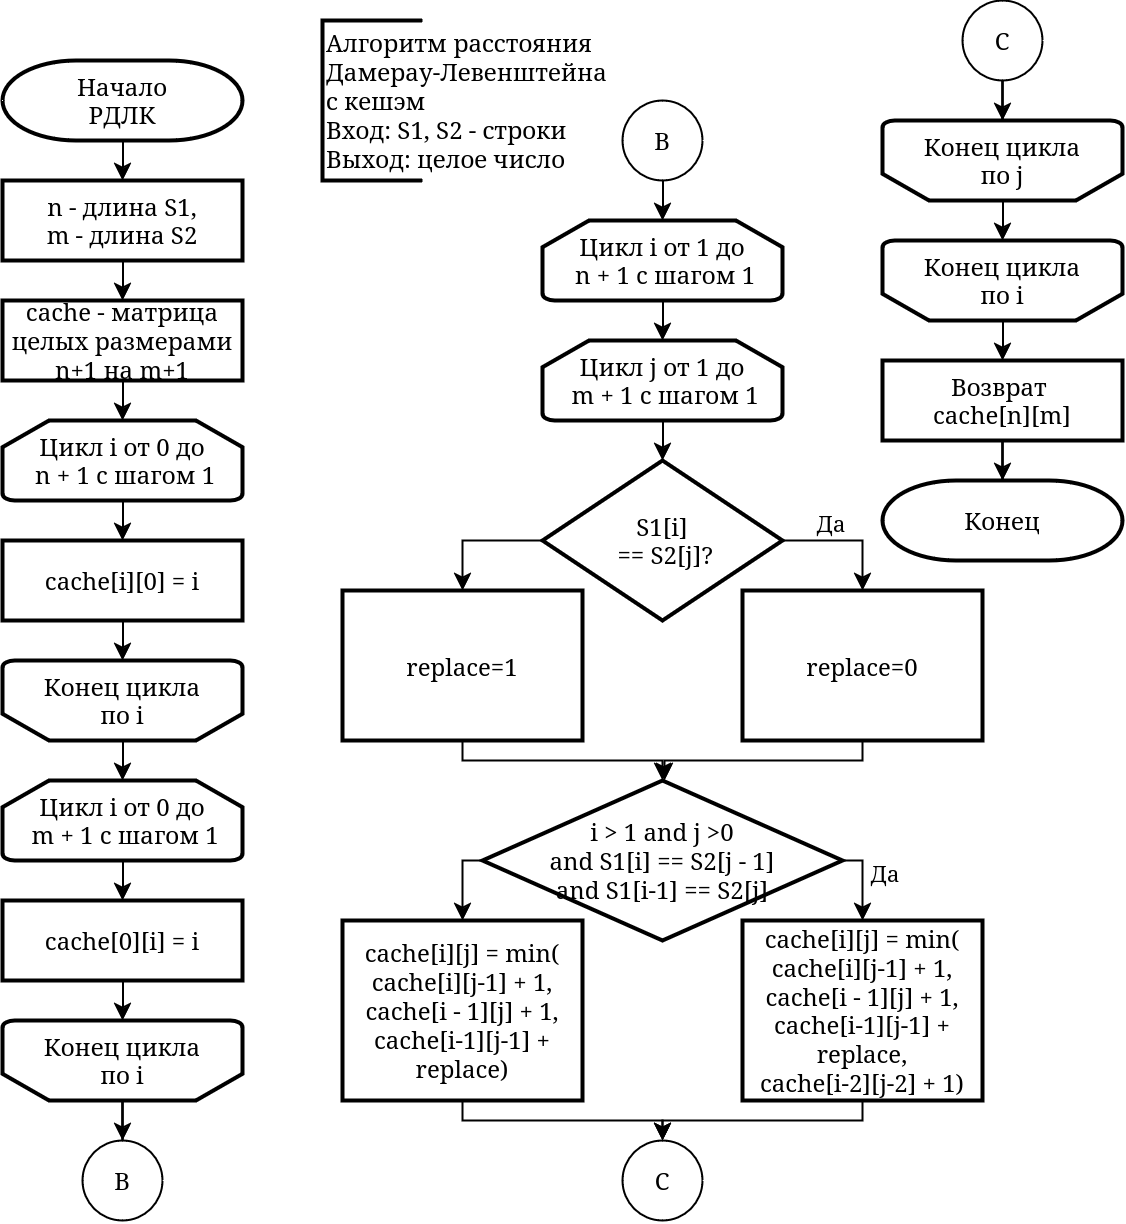
\includegraphics[width=0.9\textwidth]{RDLK}
	\caption{Схема алгоритма нахождения расстояния Дамерау-Левенштейна с кешэм}
	\label{fig:RDLK}
\end{figure}

\clearpage

\section{Вывод}

В результате конструкторской части были определены требования к ПО, а также сделаны схемы алгоритмов рекурсивного поиска расстояния Левенштейна, итерационного поиска с кешэм и итерационного алгоритма поиска расстояния Дамерау-Левенштейна с кешэм.

\clearpage
